\documentclass[12pt]{article}

\usepackage[a4paper, left=1.2in, right=1.2in]{geometry}
\usepackage{setspace}
\usepackage[utf8]{inputenc}
\usepackage[english]{babel}
\usepackage[OT1]{fontenc}
\usepackage{graphicx}
\usepackage{subcaption}
\usepackage{float}
\usepackage{fancyhdr}
\usepackage{xcolor}
\usepackage{mathtools}
\usepackage{amsmath}
\usepackage{amssymb}
\usepackage{tikz}
\usepackage{imakeidx}
\usepackage{textcomp}
\usepackage{pifont}
\usepackage{caption}
\usepackage{tabularx}
\usepackage{comment}
\usepackage{bm}
\usepackage{multirow}
\usepackage{listings}
\usepackage{longtable}
\usepackage[colorlinks=true,linkcolor=black,anchorcolor=black,citecolor=black,
            filecolor=black,menucolor=black,runcolor=black,urlcolor=black,
            backref=page]{hyperref}

%% ---- colour palette -------------------------------------------------------
\definecolor{deepblue}{rgb}{0,0,0.5}
\definecolor{deepgreen}{rgb}{0,0.5,0}

%% ---- listings setup -------------------------------------------------------
\lstset{
  language=SQL,
  morekeywords={AFTER,INSTEAD,OF,REFERENCING,FOR,EACH,ROW,DECLARE,IF,TYPE,
    NEW,OLD,RETURNS,SELF,BEGIN,END,CONSTRUCTOR,UNDER,NOT,FINAL,STATIC,
    INSTANCE,RETURN,OVERRIDING,REF,DEREF,MEMBER,FUNCTION,PROCEDURE,
    RAISE_APPLICATION_ERROR,SYSDATE,IS,ROUND,ELSIF,COMMIT,EXCEPTION,WHEN,
    OTHERS,SQLERRM,VARCHAR2,INTEGER,NUMBER,DATE,CHAR,PRIMARY,KEY,FOREIGN,
    REFERENCES,CHECK,CONSTRAINT,ON,DELETE,CASCADE,SET,NULL,UNIQUE,INTO,
    FROM,WHERE,SELECT,INSERT,UPDATE,VALUES,COUNT,DISTINCT,ADD_MONTHS,
    OPEN,SYS_REFCURSOR,OUT,IN,AS,AUTHID,CURRENT_USER,EXECUTE,IMMEDIATE,
    LOOP,END,FORCE,DROP,CREATE,INDEX,OR,TABLE,OF,OBJECT,UNDER,REPLACE,
    BEFORE,AFTER,FOLLOWS,COMPOUND,STATEMENT,DBMS_XPLAN,DISPLAY,
    EXPLAIN,PLAN,AUTOTRACE,SERVEROUTPUT},
  framesep=1pt,
  xleftmargin=0pt,
  framexleftmargin=0pt,
  frame=tb,
  framerule=1pt,
  breaklines=true,
  commentstyle=\color{deepgreen},
  keywordstyle=\color{deepblue},
  showstringspaces=false,
  basicstyle=\footnotesize\ttfamily,
  mathescape
}

\renewcommand{\tablename}{Table}
\renewcommand{\figurename}{Figure}

% ============================================================================
\begin{document}
% ============================================================================

%% ---------------------------------------------------------------------------
%%  TITLE PAGE
%% ---------------------------------------------------------------------------
\begin{titlepage}
  \begin{center}
    \vspace*{1cm}
    {\large COMPUTER SCIENCE DEPARTMENT}\\[0.4cm]
    {\large Computer Science -- Curriculum Artificial Intelligence}\\[0.3cm]
    \hrulefill\\[0.4cm]
    {\large Project Assignment -- Database Systems}\\[0.6cm]
    {\LARGE \textbf{StageUp}}\\[0.2cm]
    {\Large Audiovisual Equipment Booking System}\\[0.3cm]
    {\large Database Design and Implementation}\\[1cm]
    \hrulefill\\[0.5cm]
    \begin{tabularx}{\textwidth}{@{}Xr@{}}
      {\large Student:} & {\large \textit{Valerio Flavio}} \\
    \end{tabularx}
    \vfill
    {\large Academic Year 2025/2026}
  \end{center}
\end{titlepage}

\tableofcontents
\newpage

% ============================================================================
\section{Conceptual Design}
% ============================================================================

\subsection{Requirements}

\begin{table}[H]
  \renewcommand{\arraystretch}{1.3}
  \begin{tabularx}{\textwidth}{|X|}
  \hline
  \multicolumn{1}{|c|}{\textbf{``StageUp'' -- Audiovisual Equipment Booking System}} \\ \hline
  The company ``StageUp'' has a central office and several operational depots located across the world,
  each covering a specific region, which consists of one or more municipalities, where they manage the
  rental and installation of audiovisual equipment for events. The central office does not handle
  physical setups. Both the central office and depots are characterized by name, address,
  city/province, and number of employees. Bookings, either recurring or one-time, are coordinated by
  the central office. Bookings can be placed by customers via phone, postal mail, email, or through the
  website. Besides one-time bookings, the company also handles seasonal contracts and special
  promotional rentals. Bookings are delivered and installed at customer event locations, which are
  characterized by address, house number, postal code, city, and province. Since each customer can have
  one or more event locations, each address is identified by a unique code within the customer's
  profile. Additionally, each event location has a setup time estimate and equipment capacity. Depots
  have one or more setup teams, each with a maximum number of members. Each team is characterized by
  an identification code, a name, the number of installations made, and some personal data of its team
  members. Each booking is characterized by type, date, duration, cost, the team that handled it, and
  the details of the customer who placed it. Customers, classified as individuals or companies, are
  identified by an alphanumeric code and their personal details. \\ \hline
  \end{tabularx}
  \caption{Requirements}
\end{table}

\subsection{Analysis}

\subsubsection{Reorganisation of Concepts} 

\begin{table}[H] 
\renewcommand{\arraystretch}{1.3} 
\begin{tabularx}{\textwidth}{|X|} 
\hline \multicolumn{1}{|c|}{\textbf{Depots and Central Office}} \\ \hline 
The company operates through a single central office and several operational depots scattered across the world. The central office coordinates all the bookings but does not handle physical setups. The operational depots, on the other hand, manage the actual rental and installation of the audiovisual equipment. Both the central office and the depots are characterized by a name, address, city/province, and the number of employees. Additionally, each depot is assigned to cover a specific geographic region. \\ \hline 
\end{tabularx} 
\caption{Company Facilities Concepts} 
\end{table} 

\begin{table}[H] 
\renewcommand{\arraystretch}{1.3} 
\begin{tabularx}{\textwidth}{|X|} 
\hline \multicolumn{1}{|c|}{\textbf{Team}} \\ \hline 
Each depot has one or more setup teams. A team is identified by an identification code, a name, a maximum number of members, and the number of installations made. A team operates under exactly one depot. \\ \hline 
\end{tabularx} 
\caption{Team Concepts} 
\end{table} 

\begin{table}[H] 
\renewcommand{\arraystretch}{1.3} 
\begin{tabularx}{\textwidth}{|X|} 
\hline \multicolumn{1}{|c|}{\textbf{Member}} \\ \hline 
Each team is composed of members (specialized personnel). A member has personal data such as name, surname, phone, and email. Each member belongs to exactly one setup team. \\ \hline 
\end{tabularx} 
\caption{Member Concepts} 
\end{table} 

\begin{table}[H] 
\renewcommand{\arraystretch}{1.3} 
\begin{tabularx}{\textwidth}{|X|} 
\hline \multicolumn{1}{|c|}{\textbf{Municipality}} \\ \hline 
The specific region covered by a depot consists of one or more municipalities. Each municipality is covered by exactly one depot. \\ \hline 
\end{tabularx} 
\caption{Municipality Concepts} 
\end{table} 

\begin{table}[H] 
\renewcommand{\arraystretch}{1.3} 
\begin{tabularx}{\textwidth}{|X|} 
\hline \multicolumn{1}{|c|}{\textbf{Customer}} \\ \hline 
Customers place the bookings and can be classified as individuals or companies. They are identified by a unique alphanumeric code and their personal details. A customer can own one or more event locations. \\ \hline 
\end{tabularx} 
\caption{Customer Concepts} 
\end{table} 

\begin{table}[H] 
\renewcommand{\arraystretch}{1.3} 
\begin{tabularx}{\textwidth}{|X|} 
\hline \multicolumn{1}{|c|}{\textbf{Event Location}} \\ \hline 
An event location is a venue owned by a customer where the audiovisual equipment is delivered and installed. It is characterised by address, house number, postal code, city, province, a setup time estimate, and equipment capacity. Each location is uniquely identified within the specific customer's profile. \\ \hline 
\end{tabularx} 
\caption{Event Location Concepts} 
\end{table} 

\begin{table}[H] 
\renewcommand{\arraystretch}{1.3} 
\begin{tabularx}{\textwidth}{|X|} 
\hline \multicolumn{1}{|c|}{\textbf{Booking}} \\ \hline 
A booking represents the rental and installation of equipment requested by a customer. It is characterized by a type (recurring or one-time), date, duration, cost, booking method (phone, postal mail, email, website), and contract type (one-time, seasonal, promotional). Each booking is linked to the customer who placed it, the event location where it takes place, and the specific team that handled the physical setup. \\ \hline 
\end{tabularx} 
\caption{Booking Concepts} 
\end{table}
\subsubsection{Glossary of Terms}

\begin{table}[H]
  \renewcommand{\arraystretch}{1.3}
  \begin{tabularx}{\textwidth}{|X|X|X|X|}
  \hline
  \textbf{Term} & \textbf{Description} & \textbf{Connections} & \textbf{Synonyms} \\ \hline
  Central Office     & HQ coordinating bookings; no physical setup & Booking & HQ \\ \hline
  Depot              & Operational base; manages teams in a region & Team, Municipality & Branch \\ \hline
  Region             & Geographic area covered by a depot & Depot & Territory \\ \hline
  Municipality       & Town/area covered by exactly one depot & Depot & Town, Area \\ \hline
  Team               & Setup crew belonging to one depot & Booking, Member, Depot & Crew \\ \hline
  Member             & Employee of a team & Team & Staff, Technician \\ \hline
  Customer           & Individual or company placing bookings & Booking, Event\_Location & Client \\ \hline
  Event Location     & Venue owned by a customer & Customer, Booking & Site, Venue \\ \hline
  Booking            & Audiovisual equipment installation reservation & Customer, Event\_Location, Team & Reservation, Contract \\ \hline
  \end{tabularx}
  \caption{Glossary of Terms}
\end{table}

\subsubsection{Ambiguity Resolutions}

\begin{enumerate}
  \item \textbf{Central Office and bookings}: the central office \emph{coordinates} bookings (business
        logic) but is not a direct participant in the ER relationships; the database records which team
        handles each booking, not which office coordinated it.
  \item \textbf{Region}: not a standalone entity. It is an attribute of \textit{Depot} representing
        the geographic area covered. The region is further detailed by the municipalities it covers.
  \item \textbf{Team--Depot cardinality}: ``Depots have one or more setup teams'' implies 1:N.
        Each team belongs to exactly one depot; a depot can have multiple teams.
  \item \textbf{Booking type vs contract type}: ``type'' (recurring/one-time) describes the
        scheduling pattern; ``contract type'' (one-time/seasonal/promotional) describes the commercial
        arrangement. Both are attributes of \textit{Booking}.
  \item \textbf{Number of installations}: ``number of installations made'' is an attribute of Team.
        It is a \emph{derived redundancy} (count of bookings handled) maintained automatically. 
        This is a voluntary redundancy, consequence of a frequent operation. 
\end{enumerate}

\subsubsection{Design Choice: Central Office Entity}

The Central Office was intentionally excluded from being modeled as an independent entity within the conceptual schema to ensure greater
 efficiency and a cleaner design. Since it is a single, constant organizational unit for the entire system (essentially a "singleton"), 
 translating it into a physical entity would result in the creation of a table containing only a single tuple. This would generate unnecessary 
 overhead without providing any analytical advantage.

Furthermore, because the Central Office exclusively performs logistical coordination functions and does not actively participate in physical 
field installations, its role is considered an implicit premise of the business logic. Therefore, the fundamental relationships are established 
directly between Customers, Teams, and Bookings—namely, the entities that actively participate in the transactional flows of the database.
\pagebreak
\subsubsection{Entity-Relationship Diagram}

\paragraph{SKELETON SCHEMA} \leavevmode \newline
\begin{figure}[H]
  \centering
  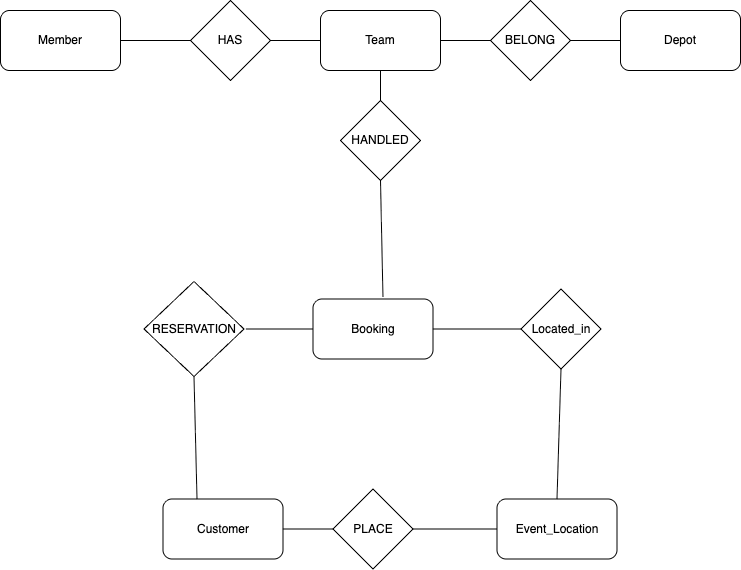
\includegraphics[width=\textwidth]{images/skeleton-er.png}
  \caption{Skeleton Schema -- Main entities and relationships (attributes and cardinalities omitted)}
\end{figure}

\noindent The skeleton schema shows the primary entities and the flow of the domain:
\textbf{Customer} $\to$ \textbf{Booking} $\to$ \textbf{Team} $\to$ \textbf{Depot}, with
\textbf{Event\_Location} connecting Customer and Booking.

\pagebreak
\paragraph{FINAL SCHEMA} \leavevmode \newline
\begin{figure}[H]
  \centering
  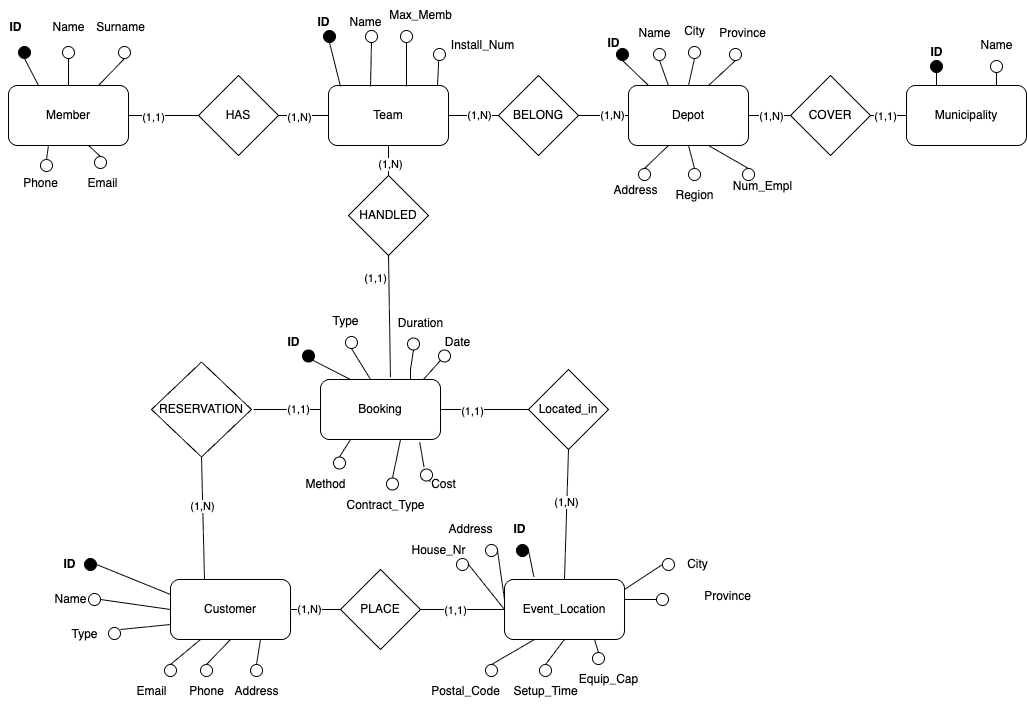
\includegraphics[width=\textwidth]{images/ER-def.png}
  \caption{Final ER Schema with all entities, attributes, cardinalities and relationships.}
\end{figure}

\subsubsection{Entities and Attributes}

\begin{table}[H]
  \renewcommand{\arraystretch}{1.3}
  \begin{tabularx}{\textwidth}{|l|X|}
  \hline
  \textbf{Entity} & \textbf{Attributes} \\ \hline
  \textbf{Depot} &
    \underline{ID} (PK), Name, Address, City, Province, Number\_Of\_Employees \\ \hline
  \textbf{Municipality} &
    \underline{ID} (PK), Name (UNIQUE), Depot\_ID (FK) \\ \hline
  \textbf{Team} &
    \underline{Code} (PK), Name, Max\_Members, Installation\_Number*,
    Depot\_ID (FK) \\ \hline
  \textbf{Member} &
    \underline{ID} (PK), Name, Surname, Phone, Email, Team\_Code (FK) \\ \hline
  \textbf{Customer} &
    \underline{ID} (PK), Name, Type $\in$ \{Individual, Company\},
    Email, Phone, Address \\ \hline
  \textbf{Event\_Location} &
    \underline{ID} (PK), Street, House\_Number, Postal\_Code, City, Province,
    Setup\_Time\_Estimate, Equipment\_Capacity, Booking\_Count*,
    Customer\_ID (FK) \\ \hline
  \textbf{Booking} &
    \underline{ID} (PK),
    Type $\in$ \{recurring, one-time\},
    Booking\_Date, Duration, Cost,
    Booking\_Method $\in$ \{phone, email, website, postal\_mail\},
    Contract\_Type $\in$ \{one-time, seasonal, promotional\},
    Team\_Code (FK), Customer\_ID (FK), Location\_ID (FK) \\ \hline
  \end{tabularx}
  \caption{Entities and Attributes (* = derived redundant attribute)}
\end{table}

\subsubsection{Relationships}

\begin{table}[H]
  \renewcommand{\arraystretch}{1.3}
  \begin{tabularx}{\textwidth}{|l|X|l|}
  \hline
  \textbf{Name} & \textbf{Semantics} & \textbf{Cardinality} \\ \hline
  COVERS & A depot covers one or more municipalities; each municipality belongs to one depot
    & Depot (1,N) -- Municipality (1,1) \\ \hline
  BELONGS\_TO & A team belongs to exactly one depot; a depot has one or more teams
    & Team (1,1) -- Depot (1,N) \\ \hline
  HAS & A team has one or more members; each member belongs to exactly one team
    & Team (1,N) -- Member (1,1) \\ \hline
  PLACE & A customer owns one or more event locations; each location belongs to one customer
    & Customer (1,N) -- Event\_Location (1,1) \\ \hline
  RESERVATION & A customer makes one or more bookings; each booking is made by one customer
    & Customer (1,N) -- Booking (1,1) \\ \hline
  LOCATED\_IN & An event location hosts one or more bookings; each booking is at one location
    & Event\_Location (1,N) -- Booking (1,1) \\ \hline
  HANDLED & A booking is handled by exactly one team; a team handles one or more bookings
    & Booking (1,1) -- Team (1,N) \\ \hline
  \end{tabularx}
  \caption{Relationships}
\end{table}

\subsubsection{Business Rules (not expressible in the ER diagram)}

\begin{enumerate}
  \item[\textbf{BR1}] Booking.Duration $> 0$; \quad Booking.Cost $\geq 0$
  \item[\textbf{BR2}] Team.Max\_Members $> 0$; \quad Team.Installation\_Number $\geq 0$
  \item[\textbf{BR3}] Depot.Number\_Of\_Employees $\geq 0$
  \item[\textbf{BR4}] Event\_Location.Setup\_Time\_Estimate $> 0$; \quad Equipment\_Capacity $\geq 0$
  \item[\textbf{BR5}] The number of members currently in a team must not exceed Team.Max\_Members.
  \item[\textbf{BR6}] Team.Installation\_Number is incremented automatically at each booking insert.
  \item[\textbf{BR7}] Event\_Location.Booking\_Count is incremented automatically at each booking insert.
\end{enumerate}

\newpage
% ============================================================================
\section{Logical Design}
% ============================================================================

\subsection{Volume Table}

The following volumes are given or derived from the problem statement.
\textit{Given}: 100 setup teams (max 10 members each), each depot operates in 10 municipalities,
1{,}000 event locations in total.
Additional volumes are estimated (marked with \dag).

\begin{table}[H]
  \scriptsize
  \renewcommand{\arraystretch}{1.3}
  \begin{tabularx}{\textwidth}{|X|X|X|X|}
  \hline
  \textbf{Concept} & \textbf{Type} & \textbf{Volume} & \textbf{Why} \\ \hline
  Depot           & E & 10         & 100 teams / 10 teams per depot \\ \hline
  Municipality    & E & 100        & 10 per depot $\times$ 10 depots (given) \\ \hline
  Team            & E & 100        & Given \\ \hline
  Member          & E & 700        & Avg 7 members/team $\times$ 100 teams \\ \hline
  Customer        & E & 500        & 1{,}000 locations / avg 2 per customer \\ \hline
  Event\_Location & E & 1{,}000    & Given \\ \hline
  Booking         & E & 100{,}000  & 300 bookings/day $\times$ 365 days (given: 300/day) (\textit{from op.2}) \\ \hline
  COVERS          & R & 100        & 1:1 cardinality with municipality \\ \hline
  BELONGS\_TO     & R & 100        & 1:1 cardinality with depot \\ \hline
  HAS             & R & 700        & 1:1 cardinality with member \\ \hline
  PLACE           & R & 1{,}000    & 1:1 cardinality with event location \\ \hline
  RESERVATION     & R & 100{,}000  & 1:1 cardinality with booking \\ \hline
  LOCATED\_IN      & R & 100{,}000  & 1:1 cardinality with booking \\ \hline
  HANDLED         & R & 100{,}000  & 1:1 cardinality with booking \\ \hline
  \end{tabularx}
  \caption{Volume Table (yearly estimates; E = entity, R = relationship)}
\end{table}

\subsection{Access Table}

\noindent\textbf{Operation 1 -- Register a new customer} (10/day)
\begin{table}[H]
  \renewcommand{\arraystretch}{1.3}
  \begin{tabularx}{\textwidth}{|X|X|X|X|}
  \hline \textbf{Concept} & \textbf{Type} & \textbf{Accesses} & \textbf{R/W} \\ \hline
  Customer & E & 1 & W \\ \hline
  \end{tabularx}
  \caption{Operation 1 -- Total: $2 \times 10 = 20$ ops/day}
\end{table}

\noindent\textbf{Operation 2 -- Record a new booking} (300/day)
\begin{table}[H]
  \renewcommand{\arraystretch}{1.3}
  \begin{tabularx}{\textwidth}{|X|X|X|X|}
  \hline \textbf{Concept} & \textbf{Type} & \textbf{Accesses} & \textbf{R/W} \\ \hline
  Customer        & E & 1 & R (verify exists) \\ \hline
  Event\_Location & E & 1 & R (verify exists) \\ \hline
  Team            & E & 1 & R (verify exists) \\ \hline
  Booking         & E & 1 & W (create booking) \\ \hline
  Booking         & E & 1 & R (retrieve new booking id) \\ \hline
  RESERVATION     & R & 1 & W (link Customer $\to$ Booking) \\ \hline
  LOCATED\_IN     & R & 1 & W (link Event\_Location $\to$ Booking) \\ \hline
  HANDLED         & R & 1 & W (link Team $\to$ Booking) \\ \hline
  Team            & E & 1 & W (Installation\_Number + 1) \\ \hline
  Event\_Location & E & 1 & W (Booking\_Count + 1) \\ \hline
  \end{tabularx}
\caption{Operation 2 -- Total: $(1+1+1+2+1+2+2+2+2+2) \times 300 = 4{,}800$ ops/day}
\end{table}
\textbf{Please note:} the accesses to update the redundant attributes (\texttt{Installation\_Number} and \texttt{Booking\_Count}) 
are included here, as they are part of the booking creation process, but they are managed by triggers and not directly by the operations.

\pagebreak

\noindent\textbf{Operation 3 -- Register a new event location} (50/day)
\begin{table}[H]
  \renewcommand{\arraystretch}{1.3}
  \begin{tabularx}{\textwidth}{|X|X|X|X|}
  \hline \textbf{Concept} & \textbf{Type} & \textbf{Accesses} & \textbf{R/W} \\ \hline
  Customer        & E & 1 & R (verify exists) \\ \hline
  Event\_Location & E & 1 & W (create location) \\ \hline
  Event\_Location & E & 1 & R (retrieve new location id) \\ \hline
  PLACE           & R & 1 & W (link Customer $\to$ Event\_Location) \\ \hline
  \end{tabularx}
  \caption{Operation 3 -- Total: $(1+2+1+2) \times 50 = 300$ ops/day}
\end{table}

\noindent\textbf{Operation 4 -- View team(s) at a specific event location} (20/day)
\begin{table}[H]
  \renewcommand{\arraystretch}{1.3}
  \begin{tabularx}{\textwidth}{|X|X|X|X|}
  \hline \textbf{Concept} & \textbf{Type} & \textbf{Accesses} & \textbf{R/W} \\ \hline
  Event\_Location & E & 1{,}000 & R (worst-case full table scan, $N$: 1{,}000) \\ \hline
  LOCATED\_IN     & R & 100     & R (avg 100 bookings per location: 100{,}000/1{,}000) \\ \hline
  Booking         & E & 100     & R (retrieve each booking) \\ \hline
  HANDLED         & R & 100     & R (traverse to team for each booking) \\ \hline
  Team            & E & 100     & R (retrieve team info) \\ \hline
  \end{tabularx}
  \caption{Operation 4 -- Total cost (assuming R=1, W=2): $(1{,}000+100+100+100+100) \times 20 = 28{,}000$ ops/day}
\end{table}

\pagebreak

\noindent\textbf{Operation 5 -- Event locations ranked by booking count descending} (5/day)
\begin{table}[H]
  \renewcommand{\arraystretch}{1.3}
  \begin{tabularx}{\textwidth}{|X|X|X|X|}
  \hline \textbf{Concept} & \textbf{Type} & \textbf{Accesses} & \textbf{R/W} \\ \hline
  Event\_Location & E & 1{,}000 & R (scan all locations) \\ \hline
  \end{tabularx}
  \caption{Operation 5 (with \texttt{Booking\_Count} redundancy) -- Total: $1{,}000 \times 5 = 5{,}000$ ops/day}
\end{table}

\subsection{Redundancy Analysis}

Two derived attributes are introduced as redundancies: \texttt{Installation\_Number} on \textbf{Team}
and \texttt{Booking\_Count} on \textbf{Event\_Location}.

\subsubsection{\texttt{Booking\_Count} on Event\_Location (for Operation 5)}

Without the redundancy, Op5 requires traversing all bookings via the \texttt{LOCATED\_IN} relationship:
\begin{table}[H]
  \renewcommand{\arraystretch}{1.3}
  \begin{tabularx}{\textwidth}{|X|X|X|X|}
  \hline \textbf{Concept} & \textbf{Type} & \textbf{Accesses} & \textbf{R/W} \\ \hline
  Event\_Location & E & 1{,}000    & R \\ \hline
  LOCATED\_IN     & R & 100{,}000  & R (traverse all bookings per location) \\ \hline
  Booking         & E & 100{,}000  & R (count all bookings) \\ \hline
  \end{tabularx}
  \caption{Op5 without \texttt{Booking\_Count}}
\end{table}
\noindent Cost Op5 without redundancy: $(1{,}000 + 100{,}000 + 100{,}000) \times 5 = 1{,}005{,}000$ ops/day.

\noindent With the redundancy, Op2 must additionally update \texttt{Booking\_Count}:
\[
  \Delta_{\text{Op2}} = 2 \times 300 = 600 \text{ ops/day extra}
\]

\noindent Total cost comparison for the five operations in the two scenarios:
\begin{itemize}
    \item \textbf{Total without redundancy:} \\
    $20 + 3{,}900 + 250 + 8{,}020 + 1{,}005{,}000 = \mathbf{1{,}017{,}190} \text{ ops/day}$

    \item \textbf{Total with redundancy:} \\
    $20 + 4{,}500 + 250 + 8{,}020 + 5{,}000 = \mathbf{17{,}790} \text{ ops/day}$
\end{itemize}

\noindent \textbf{Conclusion}: keeping \texttt{Booking\_Count} reduces the total workload by a factor
of $\sim$57. The redundancy is justified and maintained automatically by a trigger.

\subsubsection{\texttt{Installation\_Number} on Team}

Without the redundancy, computing the installation count for a specific team requires finding all bookings handled by that team. Assuming a worst-case full table scan (no indexes on the foreign keys), the database must scan the entire Booking table:
\[
  \text{Reads per query} = \text{Volume}(\text{Booking}) = 100{,}000
\]
The break-even (assuming this is queried $q$ times per day):
\[
  q \times 100{,}000 > 300 \times 2 \quad \Rightarrow \quad q > 0.006
\]
Since even a single query per day ($q = 1$) incurs $100{,}000$ reads against a maintenance penalty of only $600$ writes, keeping the redundancy is massively justified.

\subsection{Relational Schema (logical model)}

\begin{table}[H]
  \renewcommand{\arraystretch}{1.4}
  \begin{tabularx}{\textwidth}{|X|}
  \hline
  \texttt{\textbf{Customer}(\underline{ID}, Name, Type, Email, Phone, Address)} \\ \hline
  \texttt{\textbf{Event\_Location}(\underline{ID}, Street, House\_Number, Postal\_Code, City, Province,}
  \texttt{\quad Setup\_Time\_Estimate, Equipment\_Capacity, Booking\_Count*, Customer\_ID)} \\ \hline
  \texttt{\textbf{Booking}(\underline{ID}, Type, Booking\_Date, Duration, Cost, Booking\_Method,}\\
  \texttt{\quad Contract\_Type, Team\_Code, Customer\_ID, Location\_ID)} \\ \hline
  \texttt{\textbf{Team}(\underline{Code}, Name, Max\_Members, Installation\_Number*, Depot\_ID)} \\ \hline
  \texttt{\textbf{Member}(\underline{ID}, Name, Surname, Phone, Email, Team\_Code)} \\ \hline
  \texttt{\textbf{Depot}(\underline{ID}, Name, Address, City, Province, Number\_Of\_Employees, Region,}\\
  \texttt{\quad Municipalities: \{(\underline{ID}, Name)\})} \\ \hline
  \end{tabularx}
  \caption{Relational Schema (* = redundant derived attribute; \{\} = nested collection embedded in parent)}
\end{table}

\pagebreak

\subsection{UML Class Diagram}

\begin{figure}[H]
  \centering
  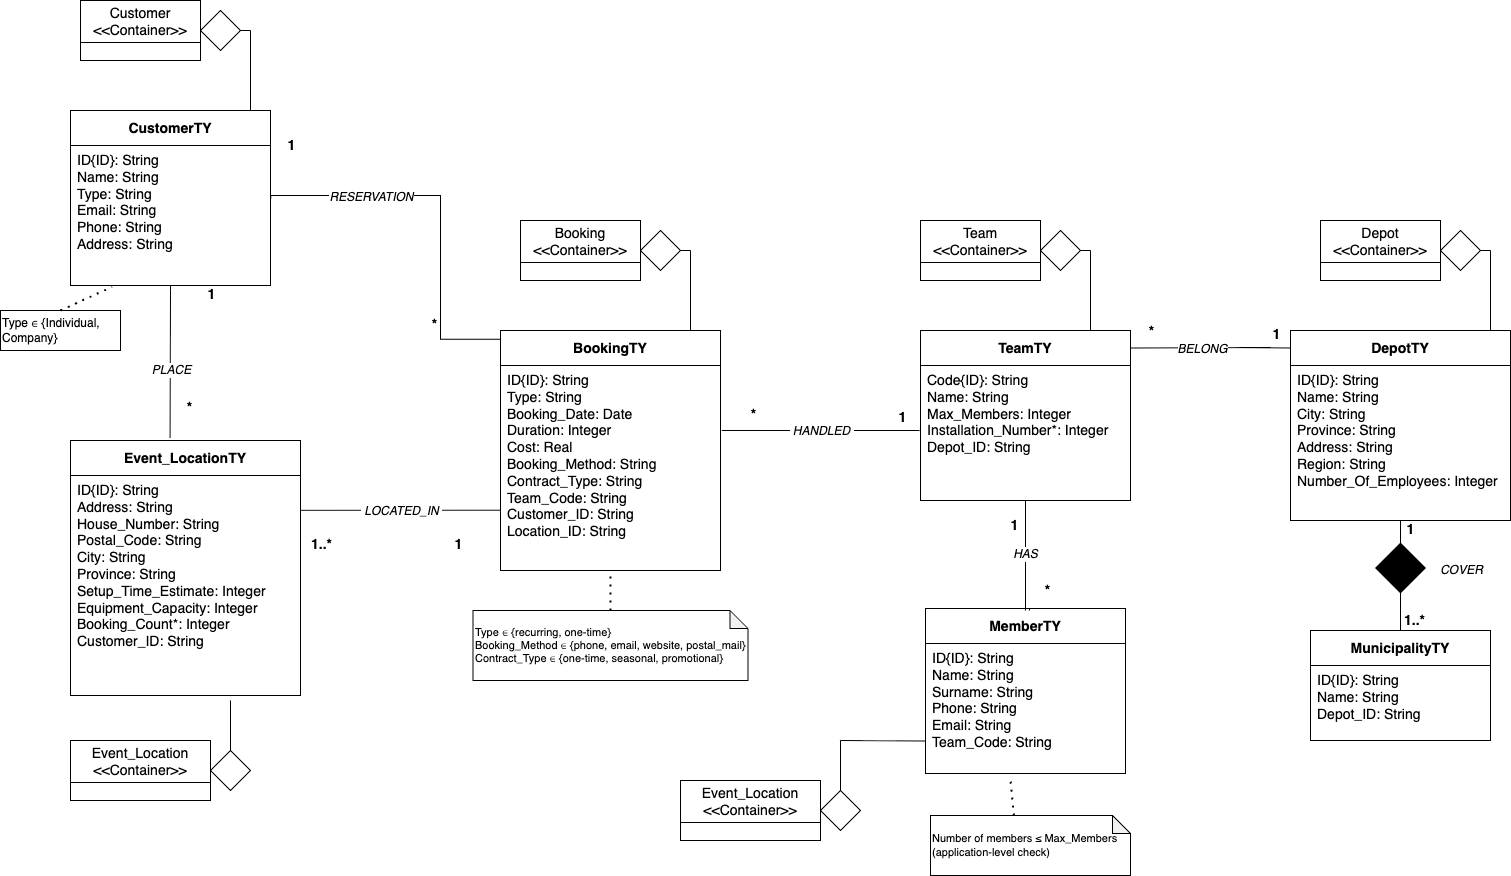
\includegraphics[width=\textwidth]{images/logic_model_uml.png}
  \caption{UML Class Diagram -- Object-Relational Logical Schema, analysis phase (exported from \texttt{Draw/logic\_model\_uml.drawio})}
\end{figure}

\subsection{Design Choices for Collections}

\subsubsection{Member -- Standalone Table (not VARRAY)}

Members could in principle be modelled as a \texttt{VARRAY} of \texttt{MemberTY} inside \texttt{TeamTY},
with a fixed size of 10 reflecting the maximum stated in the assumed value for the volume table in the second exercise.
This would make the capacity constraint self-enforcing at the storage level,
eliminating the need for a dedicated trigger.

However, this approach was intentionally rejected for the following reason:
\texttt{Team.Max\_Members} is a \emph{per-team attribute} that may vary across teams
(e.g.\ a team could have a maximum of 3, 5, or 8 members rather than always 10).
A \texttt{VARRAY(10)} would enforce only the global upper bound of the volume table,
not the declared per-team limit.
To correctly enforce \texttt{BR5}\\ ($|\text{members}| \leq \texttt{Max\_Members}$), an application-level
trigger is required regardless.
Keeping \texttt{Member} as a standalone \texttt{OF TABLE} also preserves full relational
queryability (e.g.\ finding all members of a team, or all teams a member belongs to)
without resorting to the \texttt{TABLE()} unnesting operator.

\subsubsection{Municipality -- Nested Table inside Depot}

\texttt{Municipality} is a \emph{weak entity}: it has no meaningful existence outside
its parent \texttt{Depot} (cardinality \texttt{(1,1)} on the municipality side of \texttt{COVERS}).
This makes it a natural candidate for embedding as a collection inside \texttt{DepotTY}.

A \texttt{NESTED TABLE} of \texttt{MunicipalityTY} is chosen over a \texttt{VARRAY} because
the number of municipalities per depot is unbounded in principle (the volume table gives
10 as an average, not a hard maximum), and nested tables support unbounded cardinality.
The nested table is physically stored in a separate Oracle store table
(\texttt{Municipality\_Store}) but is logically part of \texttt{Depot},
reflecting the semantic dependency correctly.

This choice eliminates the standalone \texttt{Municipality} table and the \texttt{REF DepotTY}
foreign reference that would otherwise appear in \texttt{MunicipalityTY}.
None of the five defined operations access municipalities directly,
so the restructuring has no impact on query performance or procedure logic.

\newpage
% ============================================================================
\section{Implementation}\label{sec:implementation}
% ============================================================================

This section details the physical design of the system, implementing the structures defined in the logical schema. The database is developed on \textbf{Oracle Database} utilizing the \textbf{Object-Relational} model. Each entity is structured as an Oracle \texttt{OBJECT TYPE} and persisted within an \texttt{OF TABLE}. Inter-entity relationships are established using \texttt{REF} attributes to optimize object navigation.

\subsection{Object Types}

The object types representing the primary entities of the information system are defined first. For weak entities, such as Municipalities, a nested table approach is adopted, as they do not require independent references. Robust entities are defined as standard objects with their respective attributes. Redundant attributes (e.g., \texttt{Installation\_Number} and \texttt{Booking\_Count}), identified during the performance analysis to optimize read-heavy operations, are also included.

\begin{lstlisting}
-- Municipality: element type for nested table (weak entity, no REF needed)
CREATE OR REPLACE TYPE MunicipalityTY AS OBJECT (
    ID   VARCHAR2(20),
    Name VARCHAR2(100)
);
-- Nested table type: unbounded collection of municipalities
CREATE OR REPLACE TYPE Municipality_NT AS TABLE OF MunicipalityTY;

-- Depot: embeds its municipalities as a nested table
CREATE OR REPLACE TYPE DepotTY AS OBJECT (
    ID                  VARCHAR2(20),
    Name                VARCHAR2(100),
    Address             VARCHAR2(200),
    City                VARCHAR2(100),
    Province            VARCHAR2(100),
    Number_Of_Employees INTEGER,
    Region              VARCHAR2(100),
    Municipalities      Municipality_NT
);

CREATE OR REPLACE TYPE CustomerTY AS OBJECT (
    ID      VARCHAR2(20),
    Name    VARCHAR2(100),
    Type    VARCHAR2(50),   -- 'Individual' | 'Company'
    Email   VARCHAR2(100),
    Phone   VARCHAR2(20),
    Address VARCHAR2(200)
);

-- Team belongs to exactly one Depot (1:N BELONGS_TO)
CREATE OR REPLACE TYPE TeamTY AS OBJECT (
    Code                VARCHAR2(20),
    Name                VARCHAR2(100),
    Max_Members         INTEGER,
    Installation_Number INTEGER,   -- redundancy (count of bookings handled)
    Depot               REF DepotTY
);

CREATE OR REPLACE TYPE MemberTY AS OBJECT (
    ID      VARCHAR2(20),
    Name    VARCHAR2(100),
    Surname VARCHAR2(100),
    Phone   VARCHAR2(20),
    Email   VARCHAR2(100),
    Team    REF TeamTY
);

CREATE OR REPLACE TYPE Event_LocationTY AS OBJECT (
    ID                  VARCHAR2(20),
    Street              VARCHAR2(200),
    House_Number        VARCHAR2(20),
    Postal_Code         VARCHAR2(10),
    City                VARCHAR2(100),
    Province            VARCHAR2(100),
    Setup_Time_Estimate INTEGER,
    Equipment_Capacity  INTEGER,
    Booking_Count       INTEGER,   -- redundancy (for Op5)
    Customer            REF CustomerTY
);

CREATE OR REPLACE TYPE BookingTY AS OBJECT (
    ID             VARCHAR2(20),
    Type           VARCHAR2(50),   -- 'recurring' | 'one-time'
    Booking_Date   DATE,
    Duration       INTEGER,
    Cost           NUMBER,
    Booking_Method VARCHAR2(50),   -- 'phone'|'email'|'website'|'postal_mail'
    Contract_Type  VARCHAR2(50),   -- 'one-time'|'seasonal'|'promotional'
    Team           REF TeamTY,
    Customer       REF CustomerTY,
    Location       REF Event_LocationTY
);
\end{lstlisting}

\subsection{Tables}

Following the object types definition, the corresponding typed tables are created for physical data storage. Data integrity is enforced through \texttt{PRIMARY KEY} constraints, \texttt{NOT NULL} clauses, and specific \texttt{CHECK} constraints restricting values to predefined domains. 

A critical design choice involves the referential integrity strategy, which prioritizes the preservation of historical audit trails over automated physical deletion. Destructive \texttt{ON DELETE CASCADE} policies are strictly avoided for robust entities. Specifically, the \texttt{Team} and \texttt{Depot} relationship utilizes the default \texttt{RESTRICT} behavior; this prevents the physical deletion of a depot or team if they are associated with historical bookings, enforcing a logical (soft) deletion approach at the application level to preserve service history. 

For entities that can be safely detached, the \texttt{ON DELETE SET NULL} clause is applied. This is used in the \texttt{Member} table to ensure that if a team is conceptually dissolved, its employees are merely unassigned rather than deleted. Similarly, the \texttt{Event\_Location} table utilizes \texttt{ON DELETE SET NULL} for its associated \texttt{Customer}, reflecting the business reality that a physical location persists and can be booked by other clients even if the original registering customer is removed. Conversely, the strict physical deletion of \texttt{Municipalities} tied to a \texttt{Depot} is handled natively and automatically by Oracle's nested table architecture without requiring explicit cascade commands.

\begin{lstlisting}
-- Depot: municipalities embedded as nested table (weak entity)
CREATE TABLE Depot OF DepotTY (
    ID   PRIMARY KEY,
    Name NOT NULL,
    City NOT NULL,
    Address NOT NULL,
    Number_Of_Employees NOT NULL,
    CONSTRAINT chk_depot_employees CHECK (Number_Of_Employees >= 0)
) NESTED TABLE Municipalities STORE AS Municipality_Store;

-- Team: each team belongs to exactly one Depot (1:N BELONGS_TO)
CREATE TABLE Team OF TeamTY (
    Code PRIMARY KEY,
    Name NOT NULL,
    Max_Members NOT NULL,
    CONSTRAINT chk_max_members CHECK (Max_Members > 0),
    Installation_Number NOT NULL,
    CONSTRAINT chk_installation CHECK (Installation_Number >= 0),
    Depot NOT NULL REFERENCES Depot 
);

CREATE TABLE Member OF MemberTY (
    ID      PRIMARY KEY,
    Name    NOT NULL,
    Surname NOT NULL,
    Team    REFERENCES Team ON DELETE SET NULL
);

CREATE TABLE Customer OF CustomerTY (
    ID   PRIMARY KEY,
    Name NOT NULL,
    CONSTRAINT chk_cust_type CHECK (Type IN ('Individual', 'Company')),
    Type  NOT NULL,
    Email NOT NULL
);

CREATE TABLE Event_Location OF Event_LocationTY (
    ID     PRIMARY KEY,
    Street NOT NULL,
    City   NOT NULL,
    Setup_Time_Estimate NOT NULL,
    CONSTRAINT chk_setup_time CHECK (Setup_Time_Estimate > 0),
    Equipment_Capacity NOT NULL,
    CONSTRAINT chk_equip_cap CHECK (Equipment_Capacity >= 0),
    Booking_Count NOT NULL,
    CONSTRAINT chk_bk_count CHECK (Booking_Count >= 0),
    Customer REFERENCES Customer ON DELETE SET NULL
);

CREATE TABLE Booking OF BookingTY (
    ID PRIMARY KEY,
    CONSTRAINT chk_bk_type     CHECK (Type IN ('recurring','one-time')),
    CONSTRAINT chk_bk_method   CHECK (Booking_Method IN
        ('phone','email','website','postal_mail')),
    CONSTRAINT chk_ct_type     CHECK (Contract_Type IN
        ('one-time','seasonal','promotional')),
    CONSTRAINT chk_duration    CHECK (Duration > 0),
    CONSTRAINT chk_cost        CHECK (Cost >= 0),
    Type NOT NULL, Booking_Date NOT NULL,
    Duration NOT NULL, Cost NOT NULL,
    Booking_Method NOT NULL, Contract_Type NOT NULL,
    Team     NOT NULL REFERENCES Team,
    Customer NOT NULL REFERENCES Customer,
    Location NOT NULL REFERENCES Event_Location
);
\end{lstlisting}

\subsection{Stored Procedures}

To ensure business logic is handled efficiently within the database layer, stored procedures corresponding to the primary operations defined in the logical analysis are implemented. These procedures abstract the complexities of object-relational insertions and queries from the application layer. 
\\
The first procedure manages the registration of a new customer, encapsulating the physical insertion into the system and committing the transaction.
\\
\begin{lstlisting}
-- Procedure 1: Register a new customer (Operation 1)
CREATE OR REPLACE PROCEDURE proc_register_customer (
    p_id IN VARCHAR2, p_name IN VARCHAR2, p_type IN VARCHAR2,
    p_email IN VARCHAR2, p_phone IN VARCHAR2, p_address IN VARCHAR2
) AS
BEGIN
    INSERT INTO Customer VALUES (
        CustomerTY(p_id,p_name,p_type,p_email,p_phone,p_address));
    COMMIT;
END;
\end{lstlisting}
\\
The second procedure orchestrates the creation of a booking. The existence of the requested Team, Customer, and Location is actively validated before generating the order to ensure referential safety.
\\
\begin{lstlisting}
-- Procedure 2: Record a new booking (Operation 2)
CREATE OR REPLACE PROCEDURE proc_add_booking (
    p_id IN VARCHAR2, p_type IN VARCHAR2, p_date IN DATE,
    p_duration IN INTEGER, p_cost IN NUMBER,
    p_method IN VARCHAR2, p_contract_type IN VARCHAR2,
    p_team_code IN VARCHAR2, p_customer_id IN VARCHAR2,
    p_location_id IN VARCHAR2
) AS
    v_ct NUMBER; v_cc NUMBER; v_cl NUMBER;
BEGIN
    SELECT COUNT(*) INTO v_ct FROM Team          WHERE Code=p_team_code;
    SELECT COUNT(*) INTO v_cc FROM Customer       WHERE ID=p_customer_id;
    SELECT COUNT(*) INTO v_cl FROM Event_Location WHERE ID=p_location_id;
    IF v_ct=0 THEN RAISE_APPLICATION_ERROR(-20010,'Team not found'); END IF;
    IF v_cc=0 THEN RAISE_APPLICATION_ERROR(-20011,'Customer not found'); END IF;
    IF v_cl=0 THEN RAISE_APPLICATION_ERROR(-20012,'Location not found'); END IF;
    INSERT INTO Booking VALUES (BookingTY(
        p_id, p_type, p_date, p_duration, p_cost, p_method, p_contract_type,
        (SELECT REF(t) FROM Team           t WHERE t.Code=p_team_code),
        (SELECT REF(c) FROM Customer       c WHERE c.ID=p_customer_id),
        (SELECT REF(l) FROM Event_Location l WHERE l.ID=p_location_id)));
    COMMIT;
END;
-- Note: triggers trg_update_installation_count and trg_update_booking_count
--       fire automatically after the INSERT.
\end{lstlisting}
\\
When creating a new location, an associated customer is required. The third procedure handles this insertion while correctly initializing the redundant \texttt{Booking\_Count} attribute to zero.
\\
\begin{lstlisting}
-- Procedure 3: Register a new event location (Operation 3)
CREATE OR REPLACE PROCEDURE proc_register_location (
    p_id IN VARCHAR2, p_street IN VARCHAR2, p_house_num IN VARCHAR2,
    p_postal_code IN VARCHAR2, p_city IN VARCHAR2, p_province IN VARCHAR2,
    p_setup_time IN INTEGER, p_equip_cap IN INTEGER, p_customer_id IN VARCHAR2
) AS
    v_count NUMBER;
BEGIN
    SELECT COUNT(*) INTO v_count FROM Customer WHERE ID=p_customer_id;
    IF v_count=0 THEN RAISE_APPLICATION_ERROR(-20020,'Customer not found'); END IF;
    INSERT INTO Event_Location VALUES (Event_LocationTY(
        p_id,p_street,p_house_num,p_postal_code,p_city,p_province,
        p_setup_time,p_equip_cap,
        0,  -- Booking_Count initialised to 0
        (SELECT REF(c) FROM Customer c WHERE c.ID=p_customer_id)));
    COMMIT;
END;
\end{lstlisting}
\\
To satisfy reporting queries, the fourth procedure utilizes a \texttt{SYS\_REFCURSOR} alongside the \texttt{DEREF} operator to efficiently navigate from a Booking to its assigned Team, returning a distinct list of teams for a specific location.
\\
\begin{lstlisting}
-- Procedure 4: View teams that handled a specific event location (Operation 4)
CREATE OR REPLACE PROCEDURE proc_get_teams_at_location (
    p_location_id IN VARCHAR2, p_cursor OUT SYS_REFCURSOR
) AS
BEGIN
    OPEN p_cursor FOR
        SELECT DISTINCT
               DEREF(b.Team).Code AS team_code,
               DEREF(b.Team).Name AS team_name
          FROM Booking b
         WHERE b.Location = (SELECT REF(l) FROM Event_Location l
                               WHERE l.ID = p_location_id);
END;
\end{lstlisting}
\\
Finally, the fifth procedure leverages the calculated \texttt{Booking\_Count} redundancy. By pre-aggregating these values via triggers (detailed in the subsequent section), the query avoids costly real-time joins or groupings, returning a ranked list instantly.
\\
\begin{lstlisting}
-- Procedure 5: Event locations ranked by booking count descending (Operation 5)
CREATE OR REPLACE PROCEDURE proc_get_locations_ranked (
    p_cursor OUT SYS_REFCURSOR
) AS
BEGIN
    OPEN p_cursor FOR
        SELECT l.ID, l.City, l.Street, l.Booking_Count
          FROM Event_Location l
         ORDER BY l.Booking_Count DESC;
END;
\end{lstlisting}

\subsection{Triggers}

To strictly enforce the business requirements (BR) derived during the analysis phase and dynamically maintain the consistency of redundant attributes, active database rules are implemented. 

Before each member is inserted into a team, Trigger 1 reads the team's declared maximum capacity and the current count of its members. If the limit has been reached, the insertion is aborted, satisfying BR9 natively within the DBMS.

\begin{lstlisting}
-- Trigger 1: Enforce team member capacity (BR9)
CREATE OR REPLACE TRIGGER trg_member_capacity
BEFORE INSERT ON Member
FOR EACH ROW
DECLARE
    v_current_count NUMBER;
    v_max_members   NUMBER;
    v_team_code     VARCHAR2(20);
BEGIN
    SELECT t.Code, t.Max_Members INTO v_team_code, v_max_members
      FROM Team t WHERE REF(t) = :NEW.Team;
    SELECT COUNT(*) INTO v_current_count
      FROM Member m WHERE m.Team = :NEW.Team;
    IF v_current_count >= v_max_members THEN
        RAISE_APPLICATION_ERROR(-20040,
            'Error: Team ' || v_team_code ||
            ' has reached its max capacity (' || v_max_members || ').');
    END IF;
END;
\end{lstlisting}

To maintain data consistency across performance-optimized tables, Triggers 2 and 3 operate silently upon every new booking creation. Firing \texttt{AFTER INSERT}, these triggers update the redundant counters (\texttt{Installation\_Number} on the Team and \texttt{Booking\_Count} on the Location) without any application-layer intervention, fulfilling BR10 and BR11.

\begin{lstlisting}
-- Trigger 2: Increment Installation_Number after booking insert (BR10)
CREATE OR REPLACE TRIGGER trg_update_installation_count
AFTER INSERT ON Booking
FOR EACH ROW
BEGIN
    UPDATE Team t
       SET t.Installation_Number = t.Installation_Number + 1
     WHERE REF(t) = :NEW.Team;
END;
\end{lstlisting}

\begin{lstlisting}
-- Trigger 3: Increment Booking_Count after booking insert (BR11 -- Op5 redundancy)
CREATE OR REPLACE TRIGGER trg_update_booking_count
AFTER INSERT ON Booking
FOR EACH ROW
BEGIN
    UPDATE Event_Location l
       SET l.Booking_Count = l.Booking_Count + 1
     WHERE REF(l) = :NEW.Location;
END;
\end{lstlisting}
% ============================================================================
\section{Physical Design}
% ============================================================================

\subsection{Index Analysis}

Operations 1, 2, 3 access tables primarily by primary key; the implicit PK indexes are sufficient.

\subsubsection{Operation 4 -- View Teams at a Specific Event Location (20/day)}

The query for Op4 scans \texttt{Booking} filtering by the \texttt{Location} REF column:

\begin{lstlisting}
SELECT DISTINCT DEREF(b.Team).Code, DEREF(b.Team).Name
  FROM Booking b
 WHERE b.Location = (SELECT REF(l) FROM Event_Location l WHERE l.ID = :loc_id);
\end{lstlisting}

Without an index on \texttt{Booking.Location}, Oracle performs a \textbf{FULL TABLE SCAN} over all
100{,}000 bookings for each of the 20 daily executions.

\paragraph{Without index} \leavevmode \newline
\begin{figure}[H]
  \centering
  \includegraphics[width=\textwidth]{images/OldManNOIndex.png}
  \caption{AutoTrace -- Operation 4 without \texttt{idx\_booking\_location} (full table scan)}
\end{figure}

\paragraph{Index creation} \leavevmode \newline
\begin{lstlisting}
CREATE INDEX idx_booking_location ON Booking(Location);
\end{lstlisting}

\paragraph{With index} \leavevmode \newline
\begin{figure}[H]
  \centering
  \includegraphics[width=\textwidth]{images/OldManWithIndex.png}
  \caption{AutoTrace -- Operation 4 with \texttt{idx\_booking\_location} (index range scan)}
\end{figure}

With the index, Oracle limits the scan to the $\sim$100 bookings for the requested location.

\subsubsection{Operation 5 -- Ranked Locations (5/day)}

Op5 reads all 1{,}000 \texttt{Event\_Location} rows ordered by \texttt{Booking\_Count~DESC}. This is a
full scan by design (we need all rows for ranking), so an index on \texttt{Booking\_Count} is unlikely
to be used by the optimiser for small-to-medium table sizes. The primary optimisation for Op5 is the
\texttt{Booking\_Count} \textbf{redundancy} (Section~2.3), which avoids a costly join with
\texttt{Booking} (505{,}000 vs 5{,}000 ops/day).

\paragraph{Explain Plans} \leavevmode \newline
\begin{figure}[H]
  \centering
  \includegraphics[width=\textwidth]{images/ExPlan4.png}
  \caption{Explain Plan -- Operation 4 with \texttt{idx\_booking\_location}}
\end{figure}

\begin{figure}[H]
  \centering
  \includegraphics[width=\textwidth]{images/ExPlan5.png}
  \caption{Explain Plan -- Operation 5 (scan Event\_Location with Booking\_Count stored)}
\end{figure}

\subsection{Performance Summary}

\begin{table}[H]
  \renewcommand{\arraystretch}{1.3}
  \begin{tabularx}{\textwidth}{|l|X|X|}
  \hline
  \textbf{Operation} & \textbf{Without optimisation} & \textbf{With optimisation} \\ \hline
  Op4 & Full table scan on Booking ($\sim$100{,}000 rows) & Index range scan ($\sim$100 rows) \\ \hline
  Op5 & Join + count ($\sim$101{,}000 reads, ×5/day) & Scan Event\_Location only (1{,}000 reads, ×5/day) \\ \hline
  \end{tabularx}
  \caption{Performance summary for critical operations}
\end{table}

\newpage
% ============================================================================
\section{Web Interface}
% ============================================================================

The web interface is a \textbf{Flask} (Python) application that exposes the five operations defined in
Exercise~2 via a browser-based HTML frontend, communicating with Oracle Database through the
\texttt{oracledb} library.

\subsection{Architecture}

\begin{itemize}
  \item \textbf{Backend}: \texttt{app.py} -- Flask routes calling Oracle stored procedures via
        \texttt{callproc()} / \texttt{callfunc()}.
  \item \textbf{Frontend}: Jinja2 HTML templates with CSS.
  \item \textbf{Database}: Oracle XE on \texttt{localhost:1521/xe}.
\end{itemize}

\subsection{Routes}

\begin{table}[H]
  \renewcommand{\arraystretch}{1.3}
  \begin{tabularx}{\textwidth}{|l|l|X|}
  \hline
  \textbf{URL} & \textbf{Method} & \textbf{Operation} \\ \hline
  \texttt{/}                   & GET      & Homepage with links \\ \hline
  \texttt{/register\_customer} & GET/POST & Op1: Register new customer \\ \hline
  \texttt{/add\_booking}       & GET/POST & Op2: Record new booking \\ \hline
  \texttt{/register\_location} & GET/POST & Op3: Register new event location \\ \hline
  \texttt{/teams\_at\_location}& GET/POST & Op4: View teams at a location \\ \hline
  \texttt{/ranked\_locations}  & GET      & Op5: Locations ranked by booking count \\ \hline
  \end{tabularx}
  \caption{Flask routes and corresponding operations}
\end{table}

\subsection{Backend Code}

\begin{lstlisting}
# app.py - StageUp Audiovisual Equipment Booking System
from flask import Flask, render_template, request, redirect, url_for, flash
import oracledb, datetime

app = Flask(__name__)
app.secret_key = 'supersecretkey'
DB_USER='System'; DB_PASSWORD='password123'; DB_SID='localhost:1521/xe'

def get_db_connection():
    try: return oracledb.connect(user=DB_USER,password=DB_PASSWORD,dsn=DB_SID)
    except Exception as e: print("DB error:",e); return None

@app.route('/register_customer', methods=['GET','POST'])
def register_customer():
    if request.method=='POST':
        conn=get_db_connection()
        try:
            cur=conn.cursor()
            cur.callproc("proc_register_customer",[
                request.form['cust_id'], request.form['name'],
                request.form['cust_type'], request.form['email'],
                request.form['phone'],    request.form['address']])
            conn.commit(); flash("Customer registered","success")
        except oracledb.DatabaseError as e: flash(f"Error: {e}","danger")
        finally: cur.close(); conn.close()
        return redirect(url_for('index'))
    return render_template('register_customer.html')

@app.route('/add_booking', methods=['GET','POST'])
def add_booking():
    if request.method=='POST':
        d=datetime.datetime.strptime(request.form['booking_date'],'%Y-%m-%d').date()
        conn=get_db_connection()
        try:
            cur=conn.cursor()
            cur.callproc("proc_add_booking",[
                request.form['booking_id'], request.form['btype'], d,
                int(request.form['duration']), float(request.form['cost']),
                request.form['method'],       request.form['contract_type'],
                request.form['team_code'],    request.form['customer_id'],
                request.form['location_id']])
            conn.commit(); flash("Booking recorded","success")
        except Exception as e: flash(f"Error: {e}","danger")
        finally: cur.close(); conn.close()
        return redirect(url_for('index'))
    return render_template('add_booking.html')

@app.route('/register_location', methods=['GET','POST'])
def register_location():
    if request.method=='POST':
        conn=get_db_connection()
        try:
            cur=conn.cursor()
            cur.callproc("proc_register_location",[
                request.form['location_id'], request.form['street'],
                request.form['house_number'],request.form['postal_code'],
                request.form['city'],        request.form['province'],
                int(request.form['setup_time']),int(request.form['equip_capacity']),
                request.form['customer_id']])
            conn.commit(); flash("Location registered","success")
        except Exception as e: flash(f"Error: {e}","danger")
        finally: cur.close(); conn.close()
        return redirect(url_for('index'))
    return render_template('register_location.html')

@app.route('/teams_at_location', methods=['GET','POST'])
def teams_at_location():
    teams=[]; location_id=None
    if request.method=='POST':
        location_id=request.form.get('location_id')
        conn=get_db_connection()
        try:
            cur=conn.cursor()
            out_cursor=cur.var(oracledb.CURSOR)
            cur.callproc("proc_get_teams_at_location",[location_id,out_cursor])
            teams=out_cursor.getvalue().fetchall()
        except Exception as e: flash(f"Error: {e}","danger")
        finally: cur.close(); conn.close()
    return render_template('teams_at_location.html',
                           teams=teams, location_id=location_id)

@app.route('/ranked_locations')
def ranked_locations():
    locations=[]; conn=get_db_connection()
    try:
        cur=conn.cursor()
        out_cursor=cur.var(oracledb.CURSOR)
        cur.callproc("proc_get_locations_ranked",[out_cursor])
        locations=out_cursor.getvalue().fetchall()
    except Exception as e: flash(f"Error: {e}","danger")
    finally: cur.close(); conn.close()
    return render_template('ranked_locations.html',locations=locations)

if __name__=='__main__': app.run(debug=True)
\end{lstlisting}

\subsection{Frontend Screenshots}

\begin{figure}[H]
  \centering
  \includegraphics[width=0.85\textwidth]{images/HomePage.png}
  \caption{Homepage}
\end{figure}

\begin{figure}[H]
  \centering
  \includegraphics[width=0.85\textwidth]{images/Op1.png}
  \caption{Operation 1 -- Register a new customer}
\end{figure}

\begin{figure}[H]
  \centering
  \includegraphics[width=0.85\textwidth]{images/Op2.png}
  \caption{Operation 2 -- Record a new booking}
\end{figure}

\begin{figure}[H]
  \centering
  \includegraphics[width=0.85\textwidth]{images/Op3.png}
  \caption{Operation 3 -- Register a new event location}
\end{figure}

\begin{figure}[H]
  \centering
  \includegraphics[width=0.85\textwidth]{images/Op4.png}
  \caption{Operation 4 -- View teams that handled setups at an event location}
\end{figure}

\begin{figure}[H]
  \centering
  \includegraphics[width=0.85\textwidth]{images/Op5.png}
  \caption{Operation 5 -- Event locations ranked by booking count (descending)}
\end{figure}

\end{document}
